% label prefix for this part: pm

\chapter{Projektmanagement}

\section{Vorgehensmodell}

Das gesamte Projekt wurde im Stil von \gls{rup} geführt und dementsprechend in die vier Phasen Inception, Elaboration, Construction und Transition aufgeteilt. Eine Übersicht über den Projektverlauf ist in der Abbildung \ref{fig:pm:project_overview} zu sehen.

\begin{figure}[H]
	\centering
	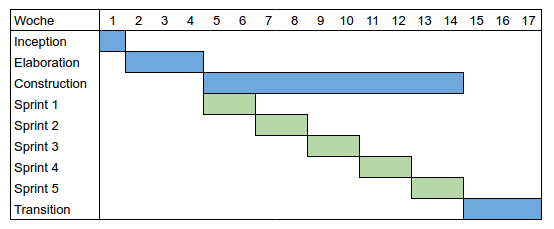
\includegraphics[width=0.8\linewidth]{fig/project_overview}
	\caption{Übersicht Projektverlauf}
	\label{fig:pm:project_overview}
\end{figure}

Die Inception-Phase diente dazu, den Auftrag zu definieren und sich gemeinsam auf klare Ziele und ein grobes Vorgehen zu einigen. Dazu kam die Installation der Infrastruktur.

In der Elaborations-Phase wurden weitere Informationen gesammelt. Ein Grossteil der Use-Cases und Arbeitspakete wurden definiert sowie das Domänenmodell erstellt. Zudem wurden die wichtigsten Risiken (Siehe auch \ref{sec:risiken}) definiert. Hauptziel war es, die Construction-Phase zu planen.

In der Construction-Phase wurde nach agiler Vorgehensweise gearbeitet, so dass der Auftraggeber die Schwerpunkte setzen und priorisieren konnte (dazu mehr in Kapitel \ref{sec:pm:sprints}. Hier wurde die fertige Applikation entwickelt.

Die Transition-Phase diente der Übergabe und Auslieferung sowie der Fertigstellung der Dokumentation.


\subsection*{Sprints} \label{sec:pm:sprints}


Es wurden in der Construction-Phase in zweiwöchigen Sprints gearbeitet. Zu Beginn fand jeweils ein Sprintplanungsmeeting mit \gls{nine} statt, wo der Plan für den kommenden Sprint diskutiert wurde und gleichzeitig eine Retrospektive auf den vergangenen Sprint abgehalten wurde.

Im Anhang (Kapitel \ref{appendix:sprints}) befinden sich die Auswertungen der einzelnen Sprints.


\section{Rollen und Verantwortlichkeiten}

An diesem Projekt arbeiten die beiden unten aufgeführten Informatik-Studenten. Aufgrund der entsprechenden Stärken und beruflichen Orientierungen übernimmt Philipp Christen die Verantwortung über das Frontend, Ueli Bosshard übernimmt die Verantwortung über das Backend und die Kommunikation mit apt.

\begin{tabularx}{\textwidth}{| X | X | }
    \hline
    \begin{minipage}{.5\textwidth}
        \begin{figure}[H]
            \centering
            
\includegraphics[width=0.6\textwidth,keepaspectratio]{fig/ubos}
            \label{fig:authors:ubos}
        \end{figure}
    \end{minipage}
	&
	\begin{minipage}{.5\textwidth}
        \begin{figure}[H]
            \centering
            
\includegraphics[width=0.6\textwidth,keepaspectratio]{fig/pchr}
            \label{fig:authors:pchr}
        \end{figure}
    \end{minipage} \\
    Ueli Bosshard & Philipp Christen \\
    Stärken: Systemtechnik, OS, Netzwerk, DB
    &
    Stärken: Web-Entwicklung, Frontend, UX, Mockups \\
    \hline
\end{tabularx}

\section{Risiken}\label{sec:risiken}

Um die potentiellen Risiken während des Projekts zu sammeln, wurde eine Risiko-Checkliste verwendet. Für jedes Risiko wurde ein zusätzlicher Aufwand in Stunden geschätzt, welcher anfallen würde wenn das Risiko eintritt. Multipliziert mit der geschätzten Eintrittswahrscheinlichkeit ergab dies einen gewichteten Mehraufwand. Dieser wurde in fünf Kategorien (sehr gering bis sehr schwer) eingestuft.

Ziel war es, alle Risiken bis Ende Elaborations-Phase entweder komplett auszuschliessen oder soweit zu entschärfen, dass beim Eintreten Sicherheitsmassnahmen greifen und keine grosse Verzögerung oder anderen Schaden verursacht werden.

Es wurden nur für das Projekt relevante Risiken analysiert. Risiken wie 'Krankheit' wurden absichtlich nicht notiert, da es hier keine sinnvollen Präventionsmassnahmen gibt.

\begin{landscape}
\begin{table}[H]
\caption{Alle berücksichtigten Risiken}
\label{tab:risikoanalyse}
\begin{tabular}{|l|p{4cm}|l|l|l|l|p{5cm}|p{5cm}|}
\hline
ID  & Risiko                                                        & SP\footnotemark[1] & EW\footnotemark[2]   & SG\footnotemark[3]  & Gewichtung                          & Präventionsmassnahmen                                                                            & Massnahme bei Eintritt                                                                     \\ \hline
R01 & Regelwerk zwischen Updates und Systemen zu komplex            & 40 & 25\% & 10  & \cellcolor[HTML]{FE0000}Sehr Schwer & Klare Anforderungen definieren, Erwartungen des Auftraggebers früh abholen.                      & Einschränken der Anforderungen.                                                            \\
R02 & Komplexes Permission-System für Benutzer                      & 24 & 25\% & 6   & \cellcolor[HTML]{FD6864}Schwer      & In Elaborations-Phase auf Rechtesystem einigen, so dass Machbarkeit gewährleistet ist.           & Anforderungen einschränken oder komplett weglassen.                                        \\
R03 & Ruby für Agent-Umsetzung oder Anschluss an apt nicht geeignet & 16 & 25\% & 4   & \cellcolor[HTML]{FFCB2F}Mittel      & So früh wie möglich Eignung von Ruby für Agent überprüfen.                                       & Python benutzen, wo es ähnliche Projekte gibt.                                             \\
R04 & apt-Schnittstelle weniger umfangreich als erwartet            & 4  & 50\% & 2   & \cellcolor[HTML]{009901}Gering      & Frühzeitiges Abklären des Umfangs der apt-Schnittstelle.                                         & Selbst erstellte Schnittstelle einsetzen oder Aufgabe anpassen, falls nicht anders lösbar. \\
R05 & Zertifikat-Handling ist komplexer als erwartet                & 8  & 10\% & 0.8 & \cellcolor[HTML]{34FF34}Sehr Gering & Machbarkeit früh abklären.                                                                       & Spezialisten\footnotemark[4] anfragen. \\
R06 & Control Center durch gleichzeitige Anfragen überfordert       & 16 & 25\% & 4   & \cellcolor[HTML]{009901}Gering      & Auslastung einplanen, mit erstem stabilem Prototypen Last-Tests fahren.                   & Spezialisten\footnotemark[4] anfragen. \\
R07 & Auftraggeber mit Umsetzung unzufrieden                        & 24 & 25\% & 6   & \cellcolor[HTML]{FD6864}Schwer      & Use-Cases, Scope und NFAs früh bestätigen lassen. Regelmässige Meetings mit gemeinsamer Planung. & Meeting mit Betreuer und Auftraggeber einberufen.                                          \\ \hline
\end{tabular}
\end{table}


\footnotetext[1]{Schadenspotenzial (h)}
\footnotetext[2]{Eintrittswahrscheinlichkeit (\%)}
\footnotetext[3]{Schaden gewichtet (h)}
\footnotetext[4]{\gls{nine} oder Prof. Steffen (HSR)}

\end{landscape}

\subsection*{Kritische Risiken}

Die besonders kritischen Risiken werden hier kurz erläutert und genauer beschrieben.

\newcommand{\projectrisk}[4]{
	\begin{tabularx}{\linewidth}{lX}
		\toprule
		\textbf{Risiko} & #1\\
		\midrule
		\textbf{Titel} & #2\\
		\textbf{Beschreibung} & #3\\
		\textbf{Prävention/Massnahme} & #4\\
		\bottomrule
	\end{tabularx}
}


\projectrisk{R01}{Regelwerk zwischen Updates und Systemen zu komplex}
{Es war von Beginn an nicht klar, wie das Regelwerk genau aussehen soll, welches die Kombinationen von Systemen und Updates einschränkt. Im schlimmsten Fall können es beliebig tiefe Abhängigkeiten sein, welche über mehrere Gruppen hinweg geprüft werden müssen.}
{In der Elaborations-Phase sollte so gut wie möglich geklärt werden, in welcher Form das Regelwerk entstehen soll. Sobald sich herausstellt, dass die gewählte Tiefe der Umsetzung zu viel Aufwand verursacht, wird mit dem Auftraggeber entschieden, ob die Anforderung gegebenenfalls eingegrenzt werden kann.}


\projectrisk{R02}{Komplexes Permission-System für User}
{Wie beim Regelwerk zwischen Updates und Systemen können die Berechtigungen der Benutzer beliebig fein konzeptioniert werden. Dadurch müssen nicht nur die Berechtigungen selbst geprüft werden, sondern auch Abhängigkeiten unter den Berechtigungen - es ist sinnlos, wenn man einem Benutzer das Updaten einer spezifischen Gruppe verbietet, aber das Erstellen und Bearbeiten einer Gruppe erlaubt ist.}
{Wiederum soll in der Elaboration-Phase mit dem Auftraggeber das Rechtesystem vereinbart werden um die Machbarkeit zu gewährleisten. Falls dies nicht gelingt oder sich als schwerer als geplant entpuppt, sollen wenn möglich die Anforderungen eingeschränkt werden. Falls es keine brauchbare Lösung gibt, muss auf das Rechtesystem verzichtet werden.}


\projectrisk{R07}{Auftraggeber mit Umsetzung nicht zufrieden}
{Der Auftraggeber kann trotz korrekter Umsetzung mit dem Endresultat nicht zufrieden sein, etwa indem implizite und nicht dokumentierte Annahmen von Kundenseite her nicht oder nur teils erfüllt wurden.}
{Es soll früh abgegrenzt werden, was genau zum Projektumfang gehört, welche Use-Cases und NFAs gelten und welche Features implementiert werden. Dies soll vom Auftraggeber bestätigt werden. Regelmässige Meetings mit Statusbesprechung und Planung der nächsten Wochen sollen unterschiedliche Vorstellungen verhindern und alle Parteien am Entstehungsprozess beteiligen lassen. Falls trotzdem Unzufriedenheit auftreten sollte, muss dies zusammen mit dem Betreuer genauer angeschaut werden.}

\subsection*{Risikoüberwachung}

Die kritischen Risiken R01 und R02 konnten entschärft werden. Das Regelwerk (R01) wurde zusammen mit dem Auftraggeber als zu komplex angesehen und hätte den Rahmen des Projekts gesprengt. Die Abklärungen und Vorschläge wurden im Ausblick (Kapitel \ref{sec:ausblick:regelwerk}) erwähnt.

Das Permission-System für die Benutzer (R02) wurde vereinfacht und als Rechte-Skala (PermissionLevel, siehe auch Kapitel \ref{sec:domain:permission_level}) definiert. Dies erfüllt die Anforderungen an das Feature, aber ist weniger komplex umzusetzen als alternative Lösungen (siehe dazu die Mockups in Kapitel \ref{sec:design:permissions}).

R07 wurde ebenfalls im Laufe der Arbeit minimiert. \gls{nine} wurde mindestens alle zwei Wochen über neue Erkenntnisse und Entwicklungen informiert und Feedback wurde jeweils direkt diskutiert und in den nächsten Sprint übernommen.


\section{Infrastruktur} \label{sec:pm:infrastructure}

Da es sich um ein Open-Source-Projekt handelt, wurde der Quellcode komplett veröffentlicht. Bereits während der Entwicklung war er jederzeit auf Github\footnote{\purl{https://github.com/upd89/}} einsehbar.

Entwickelt wurde primär mit VIM\footnote{\purl{http://www.vim.org/}}, Atom\footnote{\purl{https://atom.io}} oder RubyMine\footnote{\purl{
https://www.jetbrains.com/ruby}}. Bei jedem Commit nach GitHub checkte Travis-CI\footnote{\purl{https://travis-ci.org/}} den neuesten Stand aus und führte alle Unit-Tests durch. Das Resultat wurde einerseits via Email an die Entwickler geschickt, aber auch auf GitHub sowie auf RedMine\footnote{\purl{https://www.redmine.org/}} angezeigt. Eine Grafische Darstellung der Abläufe befindet sich in Abbildung \ref{fig:pm:entwicklungsumgebung}.


Diagramme wurden mit Astah Professional\footnote{\purl{http://astah.net/editions/professional}} und Draw.io\footnote{\purl{https://www.draw.io/}} erstellt. Bildbearbeitungen wurden mit Gimp\footnote{\purl{https://www.gimp.org/}} oder Pinta\footnote{\purl{https://pinta-project.com/pintaproject/pinta/}} vorgenommen. Für SVGs, wie zum Beispiel dem Poster, wurde Inkscape\footnote{\purl{https://inkscape.org/en/}} verwendet.

Das Erstellen der Dokumentation fand in ShareLatex\footnote{\purl{https://www.sharelatex.com/}} statt. So konnte gleichzeitig am Dokument gearbeitet werden und es benötigte keine eigene lokale Latex-Umgebung. In regelmässigen Abständen wurden die Tex-Files auf das Dokumentations-Repo auf Github\footnote{\purl{https://github.com/upd89/doc}} committet und per Webhook wurde ein PDF-File für die Ablage automatisch generiert.

\begin{figure}[H]
	\centering
	\includegraphics[width=\linewidth]{fig/entwicklungsumgebung}
	\caption{Entwicklungsumgebung}
	\label{fig:pm:entwicklungsumgebung}
\end{figure}

Zu Testzwecken wurden von \gls{nine} 10 Server gesponsert, welche  in 3 Gruppen eingeteilt wurden: Development, Test, Demo. Jede Gruppe enthält ein Control-Center sowie 2-3 Agent-Systeme. Die Dev-Systeme dienten dem aktiven Entwickeln des Frontends sowie zum Testen von neuen Features. Auf den Test-Systemen wurden nur stabile Versionen des Control-Centers installiert und dienten mehrheitlich dem Testen der Kommunikation mit den Agents. Auf den Systemen der Gruppe Demo wurden nur getestete Versionen aufgespielt. Diese dienten als Demonstrationszweck für die Industriepartner und Betreuer.

Es wurden sowohl die eigenen Notebooks als auch die von der HSR zur Verfügung gestellten Arbeitsplätze benutzt. Daneben waren zwei VMs der HSR im Einsatz; eine für Redmine und eine für Entwicklungen und Testing der Software. Der Source Code wurde über Github verwaltet.
Für Ruby und Rails wurde angestrebt, eine möglichst aktuelle Version (Ruby 2.2 respektive Rails 4.2) zu unterstützen. Als Datenbank-System wurde PostgreSQL eingesetzt. Javascript wurde primär für kleinere Optimierungen und Erleichterungen benutzt.

\clearpage
\section{Arbeitsablauf}

Um die Qualität der abgeschlossenen Tasks zu erhöhen und sicherzustellen wurde das 'Vier-Augen-Prinzip' angewendet. Jeder Task musste, bevor dessen Status auf 'Erledigt' gesetzt wurde, vom jeweils anderen Teammitglied kontrolliert und als akzeptabel eingestuft hat. Dazu existierten unterschiedliche Bedingungen: Bei Unterstützungstasks (z.B. Dokumentation o. Ä.) wurde, wo sinnvoll, eine Liste von Akzeptanzkriterien im Task selbst definiert; bei Umsetzungstasks musste der Code über Unit-Tests getestet und gelintet\footnote{Linting ist ein Prozess zur statischen Code-Analyse um potenzielle Fehler zu finden} sein.

Der normale Workflow eines Tasks in Redmine sah deshalb folgendermassen aus:

\begin{figure}[H]
	\centering
	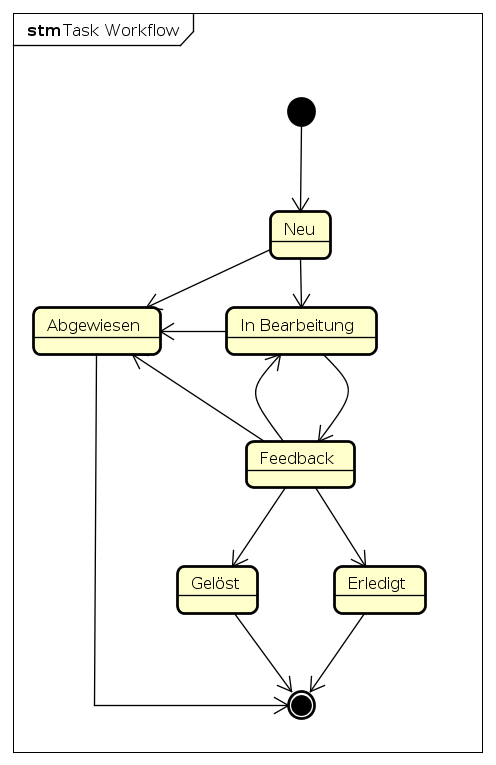
\includegraphics[width=0.5\linewidth]{fig/task_workflow}
	\caption{Workflow eines Tasks}
	\label{fig:pm:workflow}
\end{figure}

Wenn der Reviewer mit dem Resultat des Tasks nicht zufrieden war oder noch offene Punkte oder Fragen hatte, wurde der entsprechende Task wieder an den ursprünglichen Bearbeiter zurückgewiesen und in den Status 'In Bearbeitung' gesetzt. Das Feedback dazu konnte mündlich oder via Kommentar-Funktion erfolgen.

\section{Qualitätsmanagement}

\subsection*{Stil}

Um den Stil des Source-Codes einheitlich zu halten, wurde der 'Ruby On Rails Style Guide'\footnote{\purl{https://github.com/bbatsov/rails-style-guide}} angewendet. Um diesen zu prüfen und sicherzustellen wurde Rubocop\footnote{\purl{http://batsov.com/rubocop/}} eingesetzt.

\subsection*{Testing}

Wo immer sinnvoll wurden Unit-Tests für das Testen der Funktionalität verwendet. Es wurde eine Sammlung von Unit-Tests erstellt, welche die Applikation automatisch testeten.

Dabei wurde aber nicht stur der Ansatz des Test-Driven Developments verfolgt, es sollten insbesondere kritische Komponenten ausgiebig getestet werden, um die Nachhaltigkeit des Projekts sicher zu stellen.

Die Umsetzung wurde im Kapitel \ref{sec:umsetzung:testing} behandelt.

\subsection*{Usability}

Weil auch einfache Bedienbarkeit im Fokus lag, wurden Usability-Überlegungen zusammen mit dem Kunden besprochen und entsprechend umgesetzt. Es wurden auch einige Usability-Tests, primär in Form von Hallway-Testing, geplant und umgesetzt. Dies wird in Kapitel \ref{sec:umsetzung:usability} genauer beschrieben.